\documentclass{article}
\usepackage{geometry}
\usepackage{blindtext}
\usepackage[T1]{fontenc}
\usepackage[utf8]{inputenc}

\usepackage{makecell}
\usepackage{amsfonts}
\usepackage{longtable}
\usepackage{amsmath}
\usepackage{amssymb}
\usepackage{amsthm}
\usepackage{systeme}
\usepackage{graphicx}
\graphicspath{ {./images/} }

\newtheorem{theorem}{Theorem}


\setlength\parindent{24pt}

\title{Singular Value Decomposition}
\author{Vincent Mollicone, Chris Lee, Helen Chen, and Anjali Agarwal}
\date{\today}

\geometry{margin=1in, top=0.5in}

\begin{document}

\maketitle
Singular Value Decomposition (SVD) is a factorization of a matrix into 3 separate matrices that give valuable properties. We will discuss how to calculate the SVD, prove important related theorems, and explore an application of SVD called Principal Component Analysis.
\tableofcontents
\newpage

\section{Theories}
\subsection{Motivation}
The singular value decomposition, often referred to as the SVD, is a useful factorization of any matrix. Let $A\in\mathbb{R}^{m\times n}$, then the SVD of $A$ is
$$A = U \Sigma V^T$$
where $U\in\mathbb{R}^{n\times n}$ is orthonormal, $T\in\mathbb{R}^{m\times m}$ is orthonormal, and $\Sigma\in\mathbb{R}^{n\times m}$ is diagonal.

Recall from MATH 308 that if we have a symmetric matrix $A$, then we can diagonalize it with the form $A=PDP^{-1}$ where $P$ is the orthonormal eigenvectors and $D$ is diagonal. This is just a special case of the SVD, that $P = U = V$. What makes the SVD useful is that it is a sort of "diagonalization" that does not require the underlying matrix to be square.

The essence of SVD is simple. That is, having a linear transformation $A$ from $\mathbb{R}^n$ to $\mathbb{R}^m$, we want to find an orthonormal basis ($\vec{v}_i$'s) in the domain such that the image of this basis is still orthogonal (a scalar multiple of $\vec{u}_i$ where $\vec{u}_i$'s orthogonal) after the transformation $A$. Note that SVD can be preformed for complex and infinite dimensional transformations, but we will only discuss the finite, real case here. In linear algebra language, this means 
\begin{align*}
AV =A \begin{pmatrix} \vec{v}_1 & \vec{v}_2 & \cdots & \vec{v}_n  \\ \downarrow & \downarrow & &\downarrow \end{pmatrix} &= \begin{pmatrix} \sigma_1 \vec{u}_1 & \sigma_2 \vec{u}_2 & \cdots &\sigma_n \vec{u}_n  \\ \downarrow & \downarrow & &\downarrow \end{pmatrix} \\
&= \begin{pmatrix} \vec{u}_1 & \vec{u}_2 & \cdots & \vec{u}_n  \\ \downarrow & \downarrow & &\downarrow \end{pmatrix} \begin{pmatrix} \sigma_1 & 0 & \cdots & 0 \\ 0& \sigma_2 & \cdots & 0 \\ \vdots & \vdots & \ddots & \sigma_n \end{pmatrix} \\
&= U \Sigma
\end{align*}
where $\vec{v}_1, \vec{v}_2, \cdots, \vec{v}_n$ are orthonormal to each other (hence $V$ orthonormal), $\vec{u}_1, \vec{u}_2, \cdots, \vec{u}_n$ are orthonormal to each other (hence $U$ orthonormal), and $\Sigma$ is diagonal.

Since $V$ is orthogonal, $V^{-1} = V^T$, hence after rearranging we have
\begin{align*}
AV &= U \Sigma \\
AV V^{-1} &= U \Sigma V^{-1} \\
A &= U\Sigma V^T
\end{align*}
then we get the decomposition form we had for $A$.

\subsection{How to calculate SVD}
For any matrix $A$, it has been proven that $A$ can be decomposed into the form $A = U \Sigma V^T$ (where $U,V$ orthonormal and $\Sigma$ diagonal). The proof of this fact is outside the scope of these notes. However, we will show below how to actually find $U, \Sigma, V$. First, there are a few preliminary results we need to prove.
\bigskip

\textit{\textbf{Def:}} \textit{A real $n \times n$ matrix $A$ is symmetric positive semi-definite if it is symmetric (i.e. $A=A^T$) and 
$$ x^T A x \geq 0 \text{ for all nonzero vectors }x$$}
\bigskip

There are some helpful theorems we can prove about symmetric positive semi-definite matrices, which are essential for our calculation of SVD.
\bigskip

\begin{theorem}
Let $A$ be a positive semi-definite real matrix, then the eigenvalues of $A$ are non-negative.
\end{theorem} 

\begin{proof}
Let $\lambda$ be an eigenvalue of $A$ and $x$ be the corresponding eigenvector. Then 
\begin{align*}
Ax &=\lambda x \\
x^T A x &= \lambda x^Tx  = \lambda || x ||^2 
\end{align*}
Note that $x^T x$ is just a normal inner product of $x$ with itself, that is, the sum of each component square.
  
Since A is positive semi-definite, $x^T A x =\lambda ||x||^2 \geq 0$. Because the norm $||x||^2 $ is the square of a non-zero number ($x$ is an eigenvector, so must be non-zero), it must be positive. Hence: $$\lambda \geq \frac{0}{||x||^2} = 0$$
\end{proof}
\bigskip

\begin{theorem}
Let $A$ be any matrix, then $AA^T$ and $A^TA$ are symmetric positive semi-definite.
\end{theorem}

\begin{proof}
First, we will show that $AA^T$ is symmetric.

Write $$A = \begin{pmatrix} \vec{a}_1  & \rightarrow \\
\vec{a}_2 & \rightarrow \\ \vdots \\ \vec{a}_n & \rightarrow\end{pmatrix} $$
then $$A^T = \begin{pmatrix} \vec{a}_{1} & \vec{a}_{2}  & \cdots  &\vec{a}_n\\
\downarrow &\downarrow  &  & \downarrow \end{pmatrix} $$
Taking the product, we have
$$ A A^T = \begin{pmatrix} \vec{a}_1  & \rightarrow \\
\vec{a}_2 & \rightarrow \\ \vdots \\ \vec{a}_n & \rightarrow\end{pmatrix}  \begin{pmatrix} \vec{a}_{1} & \vec{a}_{2}  & \cdots  &\vec{a}_n\\
\downarrow &\downarrow  &  & \downarrow \end{pmatrix} = \begin{pmatrix} \vec{a}_1 \cdot \vec{a}_1 & \vec{a}_1 \cdot \vec{a}_2  & \cdots & \vec{a}_1 \cdot \vec{a}_n\\ \vec{a}_2 \cdot \vec{a}_1 & \vec{a}_2 \cdot \vec{a}_2 & \cdots &\vec{a}_2 \cdot \vec{a}_n \\
\vdots& \vdots & \ddots & \vdots \\
\vec{a}_n \cdot \vec{a}_1 & \vec{a}_n \cdot \vec{a}_2 & \cdots & \vec{a} _n \cdot \vec{a}_n \end{pmatrix} 
$$
Note that here $a_i \cdot a_j = a_{i1}a_{j1} + a_{i2}a_{j2} + \cdots + a_{in}a_{jn}$, so $a_i \cdot a_j = a_j \cdot a_i$, hence the above matrix is symmetric.

Now we will show that $AA^T$ is positive semi-definite. Using the formula for the transpose of a product, we can write
$$x^T AA^T x = (A^Tx)^T (A^Tx) $$

Notice that $(A^Tx)$ is just a column vector, let's call it $y$. Then we have $x^T AA^T x = y^T y = ||y||^2 \ge 0$. This shows $AA^T$ is positive semi-definite. 

Let $A \rightarrow A^T$, then the same prove will show that $A^TA$ is also positive semi-definite.
\end{proof}
\bigskip

Another theorem we will need is a theorem we have used from MATH 308. That is, 
\bigskip

\begin{theorem} Let $A$ be a $n \times n $ symmetric matrix, then we can write $A= P D P^{-1}$ where $P$ is orthonormal and have eigenvectors of $A$ as its columns, and $D$ is diagonal with eigenvalues of $A$ as diagonal entries.
\end{theorem}

\begin{proof}
(see textbook, theorem 6.19 and 6.20)
\end{proof}
\bigskip 

Now, equipped with these theorems, we can proceed to find a formula for $U, \Sigma, V$. 
\bigskip

Given $A= U \Sigma V^T$ (where $U,V$ orthonormal and $\Sigma$ diagonal), to first find $V$ and $\Sigma$, we write the following 
$$A^TA = ( U \Sigma V^T)^T ( U \Sigma V^T) = V \Sigma^T U^T U \Sigma V^T$$
It is easy to see that if $D$ is diagonal then $D^T = D$ and $D^n$ can be calculated by taking each entry to the $n$th power. Moreover, in lecture 25, we learned that if a matrix $P$ is orthonormal, then $P^{-1} = P^T$. Plugging in these relations, we have 
$$A^TA =V \Sigma^T U^T U \Sigma V^T = V \Sigma^T U^{-1} U \Sigma V^T =V \Sigma^T  \Sigma V^T = V \Sigma^2 V^{-1}$$
Since $A^TA$ is symmetric positive semi-definite by theorem 2 (in particular it is symmetric), this is just the form of diagonalization we are familiar with from 308 (theorem 3), that is, $$V = \begin{pmatrix} \vec{v}_{\lambda_1} & \vec{v}_{\lambda_2} & \cdots & \vec{v}_{\lambda_m} \end{pmatrix}, \; \Sigma^2 = \begin{pmatrix} \sigma^2_1 & 0&  \cdots & 0 \\ 0& \sigma^2_2 &\cdots & 0 \\ \vdots & \vdots & \ddots &0 \\
0 &0& \cdots & \sigma^2_m  \end{pmatrix}$$ 
where $\sigma^2_i$ are eigenvalues of $A^TA$ and $\vec{v}_{\lambda_i}$ are the corresponding normalized orthogonal eigenvectors. Notice that since $A^TA$ is positive semi-definite, the eigenvalues are non-negative (theorem 1) and so $\sigma_i \in \mathbb{R}$. So in the case where $A$ is real, we won't have $A$ mapping to a complex vector space. 
\bigskip

Similarly, we can obtain $U$ by writing,
$$AA^T = (U \Sigma V^T)(U \Sigma V^T)^T = U \Sigma V^T V \Sigma^TU^T = U \Sigma  \Sigma^TU^T = U  \Sigma^2U^{-1}$$
Then 
$$U = \begin{pmatrix} \vec{u}_{\lambda_1} & \vec{u}_{\lambda_2} & \cdots & \vec{u}_{\lambda_m} \end{pmatrix}$$ 
where $\vec{u}_{\lambda_i}$ are normalized orthogonal eigenvectors corresponding to the same set of $\Sigma^2$. One thing we have to be careful is that the order of $\vec{u}_{\lambda_i}$'s matters. They must be in the order conformed with the order of eigenvalues in $\Sigma^2$. More over, since orthonormal set of eigenvector of a matrix is not unique (multiply any of them by $-1$ will not change the orthonormality), we need to be careful with which set we pick. In the next section, we will see an example of this and how we should pick the eigenvector set $\vec{u}_i$'s.

\subsection{Consequences of the SVD}
There are several consequences of the SVD that are immensely important that we will show here. They will also come up in our application to PCA. First we define the reduced SVD.

\subsubsection{The Reduced SVD}
Let $A\in \mathbb{R}^{m\times n}$ with rank $r$. Which parts of our decomposition really matter? Recall:
\begin{align*}
    A&=U\Sigma V^T\\
    &=[ u_1 \dots u_r \mid u_{r+1} \dots u_m]\begin{bmatrix}\sigma_1 \\&&\ddots\\&&&\sigma_r\\&&&&0\\&&&&&\ddots\\&&&&&&0\end{bmatrix}\begin{bmatrix}v_1\\\vdots \\ v_r \\\hline v_{r+1}\\\vdots \\ v_n\end{bmatrix} \\
    &=[ \sigma_1u_1 \dots \sigma_ru_r \mid 0 \dots 0]\begin{bmatrix}v_1\\\vdots \\ v_r \\\hline v_{r+1}\\\vdots \\ v_n\end{bmatrix}\\
    &=[ \sigma_1u_1 \dots \sigma_ru_r]\begin{bmatrix}v_1\\\vdots \\ v_r\end{bmatrix}\\
    &= [ u_1 \dots u_r]\begin{bmatrix}\sigma_1&&0 \\&\ddots\\0&&\sigma_r\end{bmatrix}\begin{bmatrix}v_1\\\vdots \\ v_r\end{bmatrix}
\end{align*}
This gives us the following definition:
\bigskip

\paragraph{Definition:} The \underline{reduced SVD} of $A\in \mathbb{R}^{m\times n}$ with rank $r$ is the following reduced factorization of the SVD:

$$A=[ u_1 \dots u_r]\begin{bmatrix}\sigma_1&&0 \\&\ddots\\0&&\sigma_r\end{bmatrix}\begin{bmatrix}v_1\\\vdots \\ v_r\end{bmatrix}=\hat{U}\hat{\Sigma}\hat{V^\top}$$

In the reduced SVD the matrix $\Sigma$ is square matrix and $U,V^\top$ are rectangular. Note that this is opposite of the SVD where $U,V^\top$ are square and $\Sigma$ is rectangular.

\subsubsection{Rank One Decomposition}
Every matrix has multiple ways of being written as the sum of rank one matrices. For example, if $A\in\mathbb{R}^{m\times n}$ you can create $m$ rank one matrices $R_i$ by retaining row $i$ of $A$ and replacing all other entries of $A$ by 0. Then $A=R_1+\dots+R_m$ is a decomposition of A into rank one matrices. Many such rank one decompositions have no clear importance, however the SVD creates a special rank one decomposition that has many uses. The SVD allows
every matrix to be written as a positive linear combination of rank one matrices. The number of rank one
matrices in the decomposition is exactly the rank of the matrix.

\begin{theorem}
Let $A\in\mathbb{R}^{m\times n}$ be a matrix of rank $r$ and reduced SVD of the form $\hat{U}\hat{\Sigma}\hat{V^\top}$. Then $A$ admits a rank one decomposition:

$$A=\sigma_1u_1v^\top_1+\sigma_2u_2v^\top_2+\dots+\sigma_ru_rv^\top_r$$
\end{theorem}


\subsection{Examples}
We will perform the Singular Value Decomposition of the following matrix:
$$A = 
\begin{bmatrix}
4& 4\\
-3& 3\end{bmatrix}$$
First, we compute $A^TA$:
$$A^TA=\begin{bmatrix}4& -3\\4& 3\end{bmatrix} 
        \begin{bmatrix}4& 4\\-3& 3\end{bmatrix} =
        \begin{bmatrix}25& 7\\7& 25\end{bmatrix}$$ \\
Note that $\begin{bmatrix}1\\1\end{bmatrix}$ and $\begin{bmatrix}1\\-1\end{bmatrix}$ are two orthogonal eigenvectors of $A^TA$. \\ 
To get an orthonormal basis, let $v_1 = \begin{bmatrix}\frac{1}{\sqrt{2}}\\\frac{1}{\sqrt{2}}\end{bmatrix}$ and $v_2 = \begin{bmatrix}\frac{1}{\sqrt{2}}\\\frac{-1}{\sqrt{2}}\end{bmatrix}$. These have corresponding eigenvectors $(\sigma_1)^2=32, (\sigma_2)^2=18$. Thus, we have:
$$V = \begin{bmatrix}\frac{1}{\sqrt{2}}&\frac{1}{\sqrt{2}}\\\frac{1}{\sqrt{2}}&\frac{-1}{\sqrt{2}}\end{bmatrix}$$
$$\Sigma= \begin{bmatrix}\sqrt{32}& 0\\0& \sqrt{18}\end{bmatrix}= \begin{bmatrix}4\sqrt{2}& 0\\0& 3\sqrt{2}\end{bmatrix}$$ \\
Solving for $U$:
$$A = U \Sigma V^T$$
$$\begin{bmatrix}4& 4\\-3& 3\end{bmatrix} = U \begin{bmatrix}4\sqrt{2}& 0\\0& 3\sqrt{2}\end{bmatrix}
\begin{bmatrix}\frac{1}{\sqrt{2}}&\frac{1}{\sqrt{2}}\\\frac{1}{\sqrt{2}}&\frac{-1}{\sqrt{2}}\end{bmatrix}$$
$$U = \begin{bmatrix}1& 0\\0& -1\end{bmatrix}$$
So, we have computed the SVD of $A$:
$$A = U \Sigma V^T = \begin{bmatrix}1& 0\\0& -1\end{bmatrix}
\begin{bmatrix}4\sqrt{2}& 0\\0& 3\sqrt{2}\end{bmatrix}
\begin{bmatrix}\frac{1}{\sqrt{2}}&\frac{1}{\sqrt{2}}\\\frac{1}{\sqrt{2}}&\frac{-1}{\sqrt{2}}\end{bmatrix}$$

Notice that if we calculate $U$ using the same method we did to find $V$, we will find $AA^T$ has eigenvalues $\lambda = 32, 18$ and one choice of eigenvectors $\{ \vec{u}_1, \vec{u}_2 \}$  will be $\begin{pmatrix}  1 \\ 0 \end{pmatrix}, \begin{pmatrix}  0 \\ 1 \end{pmatrix}$ receptively, which is not the answer we got!? Note that if we multiply any of these eigenvectors by $-1$ it will still be a valid set of orthonormal basis. So which we should pick?

Recall from section 2.1 that we want $ A \vec{v}_i = \sigma_i \vec{u}_i$ for all $i$'s. Hence, our choice of $\vec{u}_i$ is limited by our previous choice of $\vec{v}_i$. Here, since $A\vec{v}_2= \begin{pmatrix} 0 \\  -3 \sqrt{2} \end{pmatrix}$, we need to have $\vec{u}_2 = \begin{pmatrix}   0 \\ -1 \end{pmatrix}$ (with $\sigma_2 = \sqrt{18} = 3 \sqrt{2}$), like what we got above.

\newpage
\section{Application - Principal Component Analysis}
\subsection{What Is Principal Component Analysis?}
Take a look at the following table of food consumption.

\begin{center}
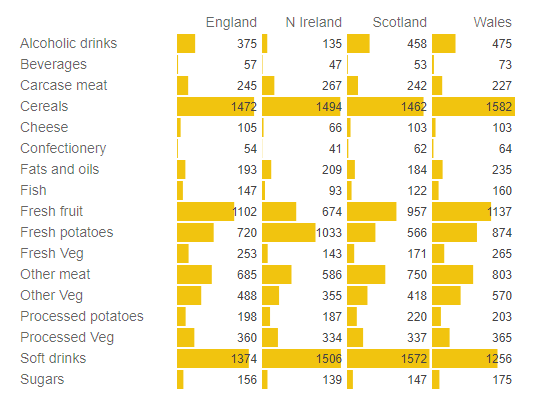
\includegraphics[width=12cm]{(17)}
\end{center}


Suppose you wanted to see if one of these countries consumes a diet that is significantly different than the others. How would you do that? At first glance they all seem very similar. You might notice some interesting variation among certain food types, but the overall variation is certainly not obvious.
\bigskip

We can use a process called principal component analysis (PCA) to help us out. PCA is a factorization used for reducing the dimensions of a multivariate data set. Furthermore, when it reduces the dimensions, it does so by projecting the total dimensions onto a lower dimensional space in such as way that preserves as much of the variability within the data as possible.

\bigskip
By applying PCA, we can reduce the 17 variables to only two. The variables, names pca 1 and pca 2 represent a two dimensional subspace that approximates the data contained in all 17 dimensions. One should note that this is different than getting ride of all but the two most important categories (such as Alcohol and Fish). Instead, each axis is a low dimension approximation so each variable could contain a combination of each of the 17 variables. We see what this means more explicitly when we learn how to compute the PCA below. The benefit of reducing the dimension in this case it we can represent a close approximation of our data on a two dimensional data set that we can easy interpret, unlike the 17 dimensional data set.
\newpage
\begin{figure}[!htp]
    \centering
    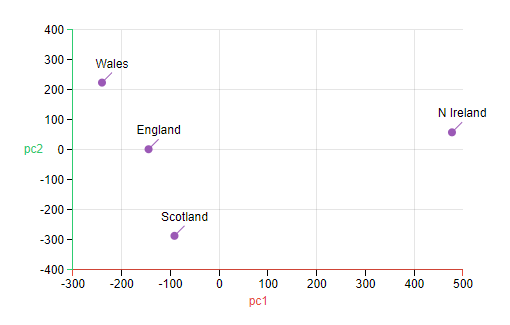
\includegraphics[width=12cm]{(18).png}
\end{figure}

Looking at our dim 2 approximation it is obvious that Northern Ireland's diet is different than the other countries. This makes sense because Northern Ireland is the only of the four countries not on the Island of Great Britain!

\subsection{How to do a Principle Component Analysis}
PCA is done using all the framework we have built up studying the SVD. In fact, PCA is simply a statistical interpretation of the SVD. It has slightly different language as the the literature for PCA uses different conventions than the SVD literature but the concepts are analogous. Let's walk through the steps to compute do the principal component analysis shown above.
\bigskip

\begin{enumerate}
\item Setting Up: First, we need to set up a matrix that contains our data. This can be easily done by simply putting the number in the spot in the matrix where it appears in the table. If we call this matrix $A$, which would be a matrix in $\mathbb{R}^{17\times 4}$, then $A_{1,1}=375$ which is the Alcoholic drinks consumed in England. By convention, the matrices for PCA have experiments (in our example we have four: England, N Ireland, Scotland, and Wales) as rows. Ours are columns so we will simply use the transpose.

\item Mean-Centering: The second set up step is called mean centering. Our data has an underlying distribution. For reasons having to do with the statistics of the PCA we want the mean of each row to be zero. This centers the underlying distribution of the data around 0. To do this we must compute the mean of each row then subtract it. This looks like:
$$~$$
Let $A$ be our data matrix. First we compute the mean for each row,
$$\bar{a}=\frac{1}{n}\sum_{j=1}^n a_j$$
$$\bar{A}=\begin{bmatrix}1\\1\\\vdots\\1\end{bmatrix}\left[~\,\bar{a}\,~\right]$$

Subtract the mean.
$$B=A-\bar{A}$$

\item The covariance matrix: Now we get what is called a covriance matrix for the rows of $B$. We will call this matrix $C$ and we get it by performing
$$C=B^\top B$$

\item The eigen-decomposition: This means we need to find the eigenvalues and eigenvectors of $C$. In particular we want to find $v_1^\top B^\top B v_1$ where $v_1$ is the largest eigenvector of of $C$ then do the same for $v_2$, $v_3$, and so on just like in the SVD. The result is that we have $$CV=VD$$ where $V$ is the eigenvectors for $C$ and $D$ is the eigenvalues.

\item Principal Components: We define the matrix of principle components of $B$ as $T$. We can equivalently define $T$ as the matrix such that,
$$T=BV$$
Recall that $B$ is our data matrix with the mean of each row subtracted off and $V$ is the eigenvectors of $C$. In PCA language, $V$ is also called the "loadings" of the principal components. The loadings are the directions of maximal variance, similar to the singular values of the SVD. In fact, in the language of the SVD, if we let $B=U\Sigma V^\top$, the SVD factorization, then we can say that,
$$T=BV=U\Sigma$$
What this means is that we can also find the PCA simply using the SVD!

\item Interpreting the Principle Components: We have the principal components, now what? What do these mean? The eigenvalues of $C$, found in step 4 (also the singular values of the SVD of $B$) represent the amount of variance captured by the particular loading $V$. In many cases most of the variance will be captured in the first few principal components. Why this is helpful is we can see the PCA as a sort of change of basis into an ordered basis where the basis vectors are ordered by how much of the data's variability thee contain. Thus what we did in our example was compute the principal components and plot them in the basis of principal components 1 and 2, dropping the others (the ones that contained the least variability). We can also explicitly compute the amount of variance contained by only considering $k$ principal components. This is done by taking the sum of the eigenvalues (singular values of SVD) of the principal components and dividing them by the total. For data set of rank $n$ matrix using only $k$ principal components this looks like,


$$\text{Var}(B)=\frac{\sum_{j=1}^{k}\lambda_j}{\sum_{j=1}^{n}\lambda_j}$$

Or equivalently in the language of the SVD,

$$\text{Var}(B)=\frac{\sum_{j=1}^{k}\sigma^2_j}{\sum_{j=1}^{n}\sigma^2_j}$$

\item Finding a Reduced Rank Matrix: Now that you have found and analyzed the principal components, say you want to keep your data in a reduced form, but put it back into the standard basis. We can also do this by the SVD. Recall that the SVD implies the existence of a useful rank one decomposition in the form,

$$B=\sigma_1u_1v^\top_1+\sigma_2u_2v^\top_2+\dots+\sigma_ru_rv^\top_r$$

To get a lower rank approximation of our data matrix using the concept of principal component analysis we can simply take the partial sum of the rank one matrices.

$$B_k=\sum_{i=1}1^k\sigma_iu_iv^\top_i$$

Note that the rank of $B_k$ is $k$. This matrix is a good approximation of $B$. In fact, $B_k$ is the "closest" rank $k$ matrix to $B$ possible (in the 2-norm). We will not prove this but see the conclusion for more information.

\item Finishing Up: Now you should have a basic idea about the concept of PCA. PCA is vastly complicated and there is more discussion that could be had about many of the parts. All these notes aim to do is give a brief introduction and give a feel for its incredible usefulness. 
\end{enumerate}

\subsection{Example problem}
Suppose we have math scores and history scores of six students. Our data points are of the form $(x_i,y_i)$ where $x_i$ denotes the math score of student $i$ and $y_i$ denotes the
history score of student $i$. After setting up and centering the data (step 1 and 2) we get,

$$\begin{bmatrix}
3& -4& 7& 1& -4& -3\\
7& -6& 8& -1& -1& -7
\end{bmatrix}$$

\noindent Compute the principal components.

\bigskip

\textbf{Solution:} We can do this easily using the SVD! First, observe that the first two steps are done for us. Let us call the matrix above $B$ to remain consistent. Thus,

$$B=\begin{bmatrix}
3&-4&7&1&-4&-3\\
7&-6&8&-1&-1&-7
\end{bmatrix}$$

Recall that we can get the principal components of $B$ directly by computing the SVD. This is what we will do. The SVD of $B$ is,

$$B=U\Sigma V^\top$$

Computing this we have,

\begin{align}
B&=U\Sigma V^\top\\
&=\begin{bmatrix}
-0.560&-0.828\\
-0.828&0.560\end{bmatrix}
\begin{bmatrix}
16.870&0\\
0&3.920
\end{bmatrix}
\begin{bmatrix}-0.443&0.427&-0.625&0.015&0.182&0.443\\
0.367&-0.013&-0.334&-0.354&0.701&-0.367\end{bmatrix}
\end{align}

(If you need a refresher about how to compute the SVD see the SVD notes)

We know from step five,

\begin{align}
T&=U\Sigma\\
&=\begin{bmatrix}
-0.560&-0.828\\
-0.828&0.560\end{bmatrix}
\begin{bmatrix}
16.870&0\\
0&3.920
\end{bmatrix}
\end{align}

Thus we have principal components
$$u_1=\begin{pmatrix}
-0.560\\
-0.828\end{pmatrix},u_2=\begin{pmatrix}
-0.828\\
0.560\end{pmatrix}$$

Looking at the singular values we see that $u_1$ contains more of the variance. We see that,

\begin{align}
\text{Var(B)}&=\frac{\sigma^2_1}{\sigma^2_1+\sigma^2_2}\\
&\approx\frac{16.870}{16.870+3.920}\\
&=\frac{16.870}{16.870+3.920}\\
&=\frac{16.870}{20.790}\\
&\approx 0.81
\end{align}

So $u_1$ contains about $81$\% of the variance.

For completeness sake, below is the calculation (in Julia) for the principal components using the sample covariance method. Note the answers are identical except for sign which makes no difference for the PCA.
\bigskip

\begin{center}
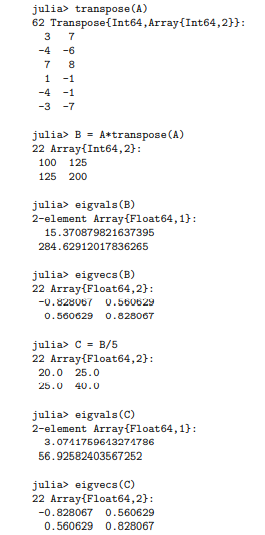
\includegraphics[width=6cm]{(19).png}
\end{center}

\newpage
\section{Conclusion and Other Applications}
So far we have reviewed what the SVD is and how to compute it. We have looked at one application of the SVD in statistics called Principal Component Analysis. However, we are only barely touching on all the possible applications of the SVD. The SVD has uses in both "pure" math and application in many other other contexts. If the this introduction to the SVD was interesting, some possible areas to go next (pertaining to the SVD of course) are:
\begin{itemize}
  \item Eckart-Young theorem. This states that our rank $k$ approximation for $B$, denoted in the notes as $B_k$ is the closest rank $k$ approximation of $B$ in the 2-norm.
  \item PCA applied to images to form a rudimentary image compression algorithm.
  \item Solving $Ax = b$ where $A$ is not a square matrix. This approach is often used in linear regression models.
  \item Google's 'PageRank' algorithm. It, as well as in other modern search engines use SVD. It is also used to find correlation patterns for recommendations on Netflix, YouTube, etc.
\end{itemize}


\end{document}
